\chapter{Research Proposal}
\label{chap:proposal}

% The goal of this work is to extend the idea of using deterministic methods to speed up Monte Carlo radiation transport to the field of geometry optimization.
% The way this is done is by applying perturbation theory to the forward and adjoint transport equations to obtain perturbed versions of the transport equations.
% The perturbed transport equations can be used to calculate the change in some response $\delta R$ due to some change in cross sections $\delta\sigma$ at some location $\vec{r}$.
% Fundamental to this methodology is that once the forward and adjoint angular fluxes are known throughout the problem domain, the results of many different perturbations can be calculated all at once, without needing to recalculate the angular flux for each perturbation.
% Thus, a significant amount of insight into possible design improvements can be obtained from a single deterministic forward and adjoint solution.

The ultimate goal of this work is to create a toolset that will automate the optimization of geometry in nuclear systems.
This toolset will use the methodology and tools described in Sections \ref{chap:dr} and \ref{chap:testprob} to calculate $\delta R$, and it will use the Dakota optimization toolkit to drive the iterative optimization of the system.

%%%%%%%%%%%%%%%%%%%%%%%%%%%%%%%%%%%%%%%%%%%%%%%%%%%%%%%%%%%%%%%%%%%%%%%%%%%%%%%%
\section{Solving Nuclear Optimization Problems}
\label{sec:proposal:solving_nuclear_optimization_problems}
%%%%%%%%%%%%%%%%%%%%%%%%%%%%%%%%%%%%%%%%%%%%%%%%%%%%%%%%%%%%%%%%%%%%%%%%%%%%%%%%

The main development challenge associated with this work will be integrating the calculation of $\delta R\left(\vec{r}\right)$ using ADVANTG with the Dakota optimization toolkit.
A single calculation of $\delta R\left(\vec{r}\right)$ provides useful information about which perturbations can be made that will improve the performance of the system, but it does not immediately provide a fully optimized solution.
$\delta R\left(\vec{r}\right)$ may need to be calculated many times for many different combinations of perturbations before an optimized solution is achieved.
The Dakota toolkit is a natural fit to use as the driver for this optimization process.

%===============================================================================
\subsection{Using $\delta R$ as Input for an Optimization Problem}
\label{sec:proposal:nuclear_optimization}
%===============================================================================

A single calculation of $\delta R\left(\vec{r}\right)$ using ADVANTG provides a mapping between the location of a perturbation and the change in the detector response.
If a change in material is made at the location $\vec{r}_1$, then the change in the detector response is equal to $\delta R\left(\vec{r}_1\right)$.
However, if another change in material is made at the location $\vec{r}_2$, then it is not quite accurate to say that the total change in the detector response is equal to $\delta R\left(\vec{r}_1\right) + \delta R\left(\vec{r}_2\right)$.
This is because the original calculation of $\delta R\left(\vec{r}\right)$ is only valid for the original geometry.

In practice, if $\vec{r}_1$ and $\vec{r}_2$ are located many path lengths away from each other, then the detector response will be very nearly equal to $\delta R\left(\vec{r}_1\right) + \delta R\left(\vec{r}_2\right)$.
This will also be true if $\vec{r}_1$ and $\vec{r}_2$ are close to each other but the magnitude of the perturbations are small.

Eventually, however, if repeated perturbations are made at points $\vec{r}_3$, $\vec{r}_4$, and beyond, then the original calculation of $\delta R\left(\vec{r}\right)$ will no longer be accurate.
$\delta R\left(\vec{r}\right)$ will need to be calculated again using ADVANTG to account for the perturbations already made.
If the goal is to optimize an entire system; e.g. find the optimal material assignments everywhere in the problem domain that results in the maximum detector response, then it is likely that $\delta R\left(\vec{r}\right)$ will need to be calculated many times.

A naive approach one might take when looking to maximize $R$ would be to calculate $\delta R\left(\vec{r}\right)$, make a change in material at its maximum value, recalculate $\delta R\left(\vec{r}\right)$, make another change in material, and repeat this process until there are no more possible perturbations left that result in an increase in $\delta R$.
This would likely result in the correct answer for problems where there are no strong local minima.
However, it would also be prohibitively computationally expensive, because a new calculation of $\delta R\left(\vec{r}\right)$ using ADVANTG would be needed for every perturbation.

Depending on the problem, it is likely that many perturbations could be made from a single calculation of $\delta R\left(\vec{r}\right)$, which would massively speed up the optimization process.
A toolkit like Dakota could be used to drive the iterative optimization process using established optimization techniques.

%===============================================================================
\subsection{Mathematical Formulation of a Nuclear Optimization Problem}
\label{sec:proposal:mathematical_formulation}
%===============================================================================

This section will describe how a simple nuclear optimization problem would be formulated in terms of the notation of a general optimization problem.
The simple nuclear optimization problem will have the following properties:
\begin{enumerate}
  \item The geometry is divided into a small volume elements, each of which have their own material.
  \item Some subset of the volume elements in the problem is available for optimization.
  \item Every volume element in the subset subject to optimization must contain some combination of materials A, B, and C.
  \item The total volume fraction of materials A, B, and C for each volume element must be equal to 1.
  \item The goal of the problem is simply to maximize the detector response.
\end{enumerate}

The mathematical formulation of a general optimization problem, shown in Equation \ref{eq:bg:opt:optimization_problem}, is repeated here:
\begin{equation*}\begin{split}
  \mbox{minimize:}  \quad & f\left(\textbf{x}\right) \\
                          & \textbf{x} \in \mathbb{R}^n \\
  \mbox{subject to:}\quad & \textbf{g}_L \leq \textbf{g}\left(\textbf{x}\right) \leq \textbf{g}_U \\
                          & \textbf{h}\left(\textbf{x}\right) = \textbf{h}_t \\
                          & \textbf{a}_L \leq \textbf{A}_i\textbf{x} \leq \textbf{a}_U \\
                          & \textbf{A}_e\textbf{x} = \textbf{a}_t \\
                          & \textbf{x}_L \leq \textbf{x} \leq \textbf{x}_U
\end{split}\end{equation*}

The \textit{design variables} $\textbf{x}$ are the volume fractions of materials A, B, and C in each volume element in the subset available for optimization.

% Since the sum of the volume fractions of materials A, B, and C is always equal to 1, if the volume fraction of material A and B are known, the volume fraction of material C is also known.
% This means that the volume fraction of material C does not need to be encoded separately.

There are \textit{constraints} on $\textbf{x}$ in the form of lower bounds $\textbf{x}_L = 0$ and upper bounds $\textbf{x}_U = 1$.
These constraints constrain the volume fractions of materials A, B, and C to be between 0 and 1.

The \textit{objective function} $f$ is equal to $-R$.
The reason it is negative is because the goal of a general optimization problem is always to minimize the objective function, while in this problem it is desired to maximize the detector response.

\textit{Linear equality constraints} are used to guarantee that the total volume fraction of materials A, B, and C in each volume element are equal to 1.
For a single volume element, the equation for the linear equality constraints $\textbf{A}_e\textbf{x} = \textbf{a}_t$ expands to
\begin{equation}
  \begin{bmatrix}1 & 0 & 0 \\ 0 & 1 & 0 \\ 0 & 0 & 1\end{bmatrix}
  \begin{bmatrix}v_A       \\ v_B       \\ v_C      \end{bmatrix} = 1,
\end{equation}
where $v_A$, $v_B$, and $v_C$ are the volume fractions of materials A, B, and C, respectively.

The simple optimization problem does not contain any nonlinear equality constraints $\textbf{h}\left(\textbf{x}\right) = \textbf{h}_t$, linear inequality constraints $\textbf{a}_L \leq \textbf{A}_i\textbf{x} \leq \textbf{a}_U$, or nonlinear inequality constraints $\textbf{g}_L \leq \textbf{g}\left(\textbf{x}\right) \leq \textbf{g}_U$.

Gradient-based optimization methods will be appropriate to solve nuclear optimization problems in this manner.
In fact, the whole point of calculating $\delta R\left(\vec{r}\right)$, as opposed to simply calculating $R$, is that $\delta R\left(\vec{r}\right)$ provides gradient information, which allows for the use of gradient-based optimization methods.

%===============================================================================
\subsection{Software Integration with Dakota}
\label{sec:proposal:software_integration_with_dakota}
%===============================================================================

There are several software development tasks that will need to be completed in order to integrate the calculation of $\delta R\left(\vec{r}\right)$ using ADVANTG with the Dakota optimization toolkit.

During the optimization process, the optimization solver will make repeated requests to calculate the objective function for various design points.
When interfacing with external programs, Dakota specifies design points by writing text files.
Thus, ADVANTG must be configured to be able to read these text files and modify the system accordingly.
ADVANTG must also be configured to provide the results of the $\delta R\left(\vec{r}\right)$ calculation in a format that is readable by Dakota.

Work will also need to be done in order to select the correct optimization algorithm and other options to be used by Dakota.

%%%%%%%%%%%%%%%%%%%%%%%%%%%%%%%%%%%%%%%%%%%%%%%%%%%%%%%%%%%%%%%%%%%%%%%%%%%%%%%%
\section{Constraints and Complex Objective Functions}
\label{sec:proposal:constraints_and_complex_objective_functions}
%%%%%%%%%%%%%%%%%%%%%%%%%%%%%%%%%%%%%%%%%%%%%%%%%%%%%%%%%%%%%%%%%%%%%%%%%%%%%%%%

Section \ref{sec:proposal:solving_nuclear_optimization_problems} describes the process for solving an optimization problem where the only goal is to minimize or maximize some response.
However, it may often be the case that the goal is more complicated than that.

Here are some examples of more complex goals:
\begin{enumerate}
  \item Maximize the difference of Responses A and B ($R_A$ and $R_B$, respectively.)
        This would be achieved by setting the objective function $f = -\left(R_A - R_B\right)$.
  \item Minimize the ratio of Responses A and B.
        This would be achieved by setting $f = R_A/R_B$.
  \item Maximize Response A while requiring Response B to be below a threshold value $t_b$.
        This could be encoded by setting \[f = \begin{cases} -R_A & \text{if } R_B < t_B \\ 0 & \text{if } R_B > t_B. \end{cases}\]
  \item Maximize the response $R$ while only allowing certain amounts of each material to exist in the problem, or while keeping the total ``cost'' of all materials below some threshold.
        These could be achieved with linear inequality constraints.
  \item Minimize the total ``cost'' of materials $C_\text{total}$ that results in a response $R$ being greater than some threshold value $R_\text{min}$.
        This could be encoded by setting \[f = \begin{cases} C_\text{total} & \text{if } R > R_\text{min} \\ \text{very large value} & \text{if } R < R_\text{min}. \end{cases}\]
\end{enumerate}

It will be necessary to add functionality to the toolset to allow for some or all of these types of goals.

%%%%%%%%%%%%%%%%%%%%%%%%%%%%%%%%%%%%%%%%%%%%%%%%%%%%%%%%%%%%%%%%%%%%%%%%%%%%%%%%
\section{Non-Fixed Source and Detector Locations}
\label{sec:proposal:moving_source_and_detector}
%%%%%%%%%%%%%%%%%%%%%%%%%%%%%%%%%%%%%%%%%%%%%%%%%%%%%%%%%%%%%%%%%%%%%%%%%%%%%%%%

Problems could be conceived where the locations of the source, detector, or both are not fixed in space.
Additional equations will need to be derived and more functionality will needed to be added to the toolset to account for these types of problems.

%%%%%%%%%%%%%%%%%%%%%%%%%%%%%%%%%%%%%%%%%%%%%%%%%%%%%%%%%%%%%%%%%%%%%%%%%%%%%%%%
\section{Calculation of $\delta R$ with Anisotropic Scattering}
\label{sec:proposal:anisotropic_scattering}
%%%%%%%%%%%%%%%%%%%%%%%%%%%%%%%%%%%%%%%%%%%%%%%%%%%%%%%%%%%%%%%%%%%%%%%%%%%%%%%%

The expression for $\delta R\left(\vec{r}\right)$ is divided into a total term $\delta R_t\left(\vec{r}\right)$ and a scattering term $\delta s\left(\vec{r}\right)$.
The full definition of the scattering term is shown in Equation \ref{eq:dr:dr_scattering_term_1} and is repeated here:
\begin{multline*}
  \delta R_s\left(\vec{r}\right) =
  \int_{4\pi}\int_0^\infty\psi^+\left(\vec{r},-\hat{\Omega},E\right) \times \\
  \left(\int_{4\pi}\int_0^\infty\delta\sigma_s\left(\vec{r},\hat{\Omega}^\prime\rightarrow\hat{\Omega},E^\prime\rightarrow E\right)\psi\left(\vec{r},\hat{\Omega}^\prime,E^\prime\right)dE^\prime d\hat{\Omega}^\prime\right)dEd\hat{\Omega}.
\end{multline*}
In order to simplify the calculation process, isotropic scattering was assumed, which resulted in Equation \ref{eq:dr:dr_scattering_term}:
\begin{equation*}
  \delta R_s\left(\vec{r}\right) =
  \int_0^\infty\phi^+\left(\vec{r},E\right)\left(\int_0^\infty\delta\sigma_s\left(\vec{r},E^\prime\rightarrow E\right)\phi\left(\vec{r},E^\prime\right)dE^\prime\right)dE.
\end{equation*}

However, there are no computational reasons why isotropic scattering must be assumed.
Denovo supports Legendre scattering expansions up to the 11th order, and most of the multigroup cross section libraries used by ADVANTG contain scattering data up to the 5th or 7th order.
Thus, it should be possible to calculate $\delta R$ without assuming isotropic scattering, and this should improve the accuracy of the results without incurring too much computational cost.

%%%%%%%%%%%%%%%%%%%%%%%%%%%%%%%%%%%%%%%%%%%%%%%%%%%%%%%%%%%%%%%%%%%%%%%%%%%%%%%%
% \section{Mixed Material Optimization}
% \label{sec:proposal:mixed_materials}
%%%%%%%%%%%%%%%%%%%%%%%%%%%%%%%%%%%%%%%%%%%%%%%%%%%%%%%%%%%%%%%%%%%%%%%%%%%%%%%%

%%%%%%%%%%%%%%%%%%%%%%%%%%%%%%%%%%%%%%%%%%%%%%%%%%%%%%%%%%%%%%%%%%%%%%%%%%%%%%%%
\section{Validation}
\label{sec:proposal:validation}
%%%%%%%%%%%%%%%%%%%%%%%%%%%%%%%%%%%%%%%%%%%%%%%%%%%%%%%%%%%%%%%%%%%%%%%%%%%%%%%%

After selecting a test problem, calculating $\delta R$, and using the toolset to produce an optimized system, it will need to be shown that the solution is actually optimal.

One way this could be done would be to use a pure Monte Carlo calculation as the simulation code used by Dakota instead of the ADVANTG-based code.
The outputs from Dakota would be the same in this case as they would be in the actual toolset; that is, the output would contain information about how the geometry and materials should be set up for the next iteration in the optimization algorithm.
However, the output from the Monte Carlo calculation would only provide the result, without the gradient information ($\delta R$) that is provided by the toolset.
This limitation means that Dakota would need to be configured to use a nongradient-based optimization method.
If the optimal solution found by the toolset is similar enough to the optimal solution found by the pure Monte Carlo-based Dakota optimization, then the toolset's solution could be taken as optimal.

It may be the case that the toolset's solution will be optimal for some problems but not optimal for others.
If non-optimal solutions are obtained, work will need to be done to determine why the toolset did not find the optimal solution and whether it can be modified to produce more optimal results in these cases.
For example, it is hypothesized that the current methodology used to calculate $\delta R$ will be sufficient for problems where the source and detector are in regions where the neutron field is nearly isotropic, whereas it will not be sufficient for problems with a great deal of anisotropy.
If a problem like this were to be encountered, one attempt that could be made to fix it would be to implement the strategy outlined in Section \ref{sec:proposal:anisotropic_scattering}.

Since a nongradient-based optimization method would need to be used for the validation, the validation will require many more simulations to produce an optimized solution compared to the toolset.
Additionally, it is expected that for some problems, each Monte Carlo simulation will have a longer runtime than the equivalent ADVANTG simulation due to the general need for Monte Carlo codes to run large numbers of particle histories in order to for them to obtain accurate results.
It would be an interesting exercise to compare the total amount of time it takes to find an optimal solution between the Monte Carlo validation and the toolset's optimization and to calculate the speedup.

%%%%%%%%%%%%%%%%%%%%%%%%%%%%%%%%%%%%%%%%%%%%%%%%%%%%%%%%%%%%%%%%%%%%%%%%%%%%%%%%
\section{Demonstration}
\label{sec:proposal:demonstration}
%%%%%%%%%%%%%%%%%%%%%%%%%%%%%%%%%%%%%%%%%%%%%%%%%%%%%%%%%%%%%%%%%%%%%%%%%%%%%%%%

After showing that the toolset can produce optimized systems for some set of small sample problems, the last step will be to demonstrate that the toolset can be used to optimize larger, more complicated systems that might be used in the real world.
Useful demonstration problems should have some the following properties:
\begin{enumerate}
  \item Geometric complexity
  \item Constraints
  \item Cost considerations
  \item Real-world applicability
\end{enumerate}
One potential demonstration problem will be described below.

%===============================================================================
\subsection{Boron Neutron Capture Therapy}
\label{sec:proposal:bnct}
%===============================================================================

The goal of the demonstration problem is to optimize a boron neutron capture therapy (BNCT) system.
BNCT is a type of radiation therapy used to treat cancer patients (most commonly those with brain tumors who had already exhausted all other potential treatments.)
In BNCT, a ${}^{10}\text{B}$-containing compound is administered to the patient, and the compound is preferentially taken up by the brain tumor.
The patient is then irradiated with neutrons, which are preferentially absorbed in the tumor due to the very high absorption cross section of ${}^{10}\text{B}$ for thermal neutrons (about 3850 barns at 0.025 eV.)
When a ${}^{10}\text{B}$ nucleus absorbs a thermal neutron, it undergoes the ${}^{10}\text{B}\left(n,\alpha\right){}^{7}\text{Li}$ reaction, which releases an alpha particle.
These alpha particles have very short path lengths in tissue (several $\mu$m), so all of their energy is deposited locally, inside the tumor.

Despite the fact that boron-10 has its highest cross section at thermal neutron energies, the neutrons used to irradiate BNCT patients are most commonly at epithermal energies.
The reason for this is that thermal neutrons do not generally penetrate deep enough into the patient to reach the brain tumor.
Epithermal neutrons penetrate deeper and thermalize within the patient's body, which results in a higher and more uniform ${}^{10}\text{B}$ reaction rate.

According to a 2001 IAEA technical document concerning the status of neutron capture therapy \cite{iaea2001}, the epithermal neutron beam should have the following characteristics for it to be useful for BNCT:
\begin{enumerate}
  \item The epithermal neutron flux (between 0.5 eV and 10 keV) should be greater than $10^9$ n/$\text{cm}^2$-s.
  \item The ratio of fast neutron flux (greater than 10 keV) to epithermal neutron flux should be less than $2\times 10^{-13}$ Gy-$\text{cm}^2$/n.
  \item The ratio of gamma dose rate to epithermal neutron flux should be less than $2\times 10^{-13}$ Gy-$\text{cm}^2$/n.
  \item The ratio of thermal neutron flux (less than 0.5 eV) to epithermal neutron flux should be less than 0.05.
  \item The ratio of total neutron current to total neutron flux should be greater than 0.7.
\end{enumerate}
The reason for the epithermal flux requirement is to decrease the irradiation time.
The reason for the beam quality requirements is to reduce undesired dose to healthy tissue.

A lightly optimized design for a BNCT system, based on a design presented in \cite{monshizadeh2015}, is shown in Figure \ref{fig:proposal:bnct_geom}.
The design has uses a DT fusion (\textasciitilde 14 MeV) neutron source with a source strength of $5\times 10^{13}$ n/s.
It uses the expensive ``FLUENTAL'' material, which is a mixture of 30\% aluminum, 69\% aluminum fluoride, and 1\% lithium fluoride by mass, as the main material in the beam shaping assembly with the purpose of lowering the high-energy source neutrons down to epithermal energies, but not to thermal energies.
It uses thin layers of cadmium and bismuth to reduce the thermal neutron and gamma population in the patient area.
It surrounds the beam shaping assembly with a large amount of lead, which acts as a epithermal neutron reflector as well as an absorber of gammas.
It contains a conical region of air between the beam shaping assembly and the patient area to obtain a more directional beam.
Lastly, it surrounds the entire assembly with thick layers of high-density borated concrete to reduce the dose to areas other than the patient area.
\begin{figure}[h!]
  \centering
  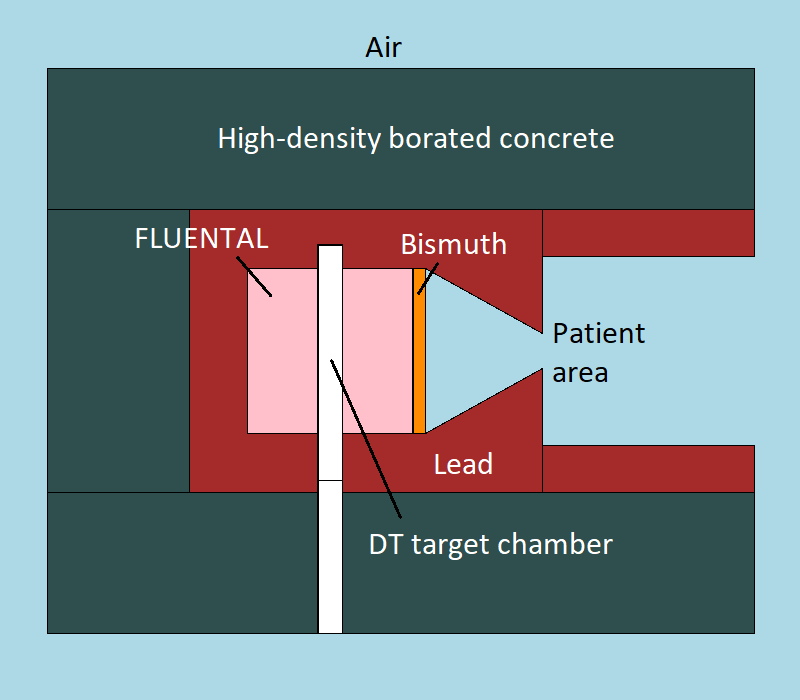
\includegraphics[width=0.75\linewidth]{content/proposal/BNCT_geom.png}
  \caption{Example geometry for a BNCT system.}
  \label{fig:proposal:bnct_geom}
\end{figure}

The design is not highly optimized.
It only contains simple types of geometry; i.e. rectangular parallelepipeds, right circular cylinders, and truncated right-angle cones (RPPs, RCCs, and TRCs in MCNP.)
No attempt was made to minimize usage of the expensive FLUENTAL material.
Table \ref{tab:proposal:bnct_metrics} shows that the design meets some of the requirements by large margins, but does not meet all requirements.
\begin{table}[h]
  \centering
  \caption{Performance metrics for the example BNCT system design.}
  \label{tab:proposal:bnct_metrics}
  \strutlongstacks{T}
  \begin{tabular}{| c | c | c | c | c |}
    \hline
    \textbf{Performance metric}                                         & \textbf{Units}     & \textbf{Value}       & \textbf{Requirement} & \Centerstack{\textbf{Meets} \\ \textbf{Requirement?}} \\ \hline
    Epithermal flux                                                     & n/$\text{cm}^2$-s  & $2.6\times 10^9    $ & > $10^9$             & True                                                  \\ \hline
    \Centerstack{Ratio of fast neutron dose \\ rate to epithermal flux} & Gy-$\text{cm}^2$/n & $7.4\times 10^{-13}$ & < $2\times 10^{-13}$ & False                                                 \\ \hline
    \Centerstack{Ratio of gamma dose        \\ rate to epithermal flux} & Gy-$\text{cm}^2$/n & $9.9\times 10^{-14}$ & < $2\times 10^{-13}$ & True                                                  \\ \hline
    \Centerstack{Ratio of thermal flux      \\ to epithermal flux     } & -                  & 0.0057               & < 0.05               & True                                                  \\ \hline
    \Centerstack{Ratio of total neutron     \\ current to flux        } & -                  & 0.62                 & > 0.7                & False                                                 \\ \hline
  \end{tabular}
\end{table}

The proposal for the demonstration problem is to use the toolset to create a more optimized design for the BNCT system.
Here are some examples of optimization problems that could be solved:
\begin{enumerate}
  \item Design a system with the maximum possible epithermal neutron flux while meeting the four beam quality metrics.
  \item Design a system with the maximum possible epithermal neutron flux while meeting the four beam quality metrics and also only containing a certain mass of FLUENTAL.
  \item Design a system that meets the epithermal flux requirement and the four beam quality metrics with the minimum possible mass of FLUENTAL.
  \item Design a system that meets the epithermal flux requirement and the four beam quality metrics with the minimum possible total system cost, where each material is assigned a cost per unit mass.
\end{enumerate}

These optimization problems would satisfy the requirements laid out at the beginning of Section \ref{sec:proposal:demonstration}.
The resultant geometries would exhibit geometric complexity, the formulations of the optimization problems would contain several types of constraints, cost considerations would be made, and the problem would be applicable to a real-world nuclear system.
